% =============================================================================
%  Diplomado en Data Science Aplicada con Python para la Toma de Decisiones
%  Clase 18: Random Forest y el Kernel Trick
%  Arca Continental Ecuador | UDLA
%
%  Compilar: pdflatex -shell-escape presentacion.tex (x2 para refs)
% =============================================================================
\documentclass[aspectratio=169, 11pt]{beamer}

\usepackage[T1]{fontenc}
\usepackage[utf8]{inputenc}
\usepackage[spanish,es-noshorthands]{babel}
\usepackage{FiraSans}
\usepackage{FiraMono}
\renewcommand{\familydefault}{\sfdefault}
\usepackage{graphicx}
\usepackage{tikz}
\usetikzlibrary{arrows.meta, positioning, shapes.geometric, shapes.misc,
  calc, fit, decorations.pathreplacing, backgrounds}
\usepackage{fontawesome5}
\usepackage{minted}
\usepackage{tcolorbox}
\tcbuselibrary{minted, skins, breakable}
\usepackage{booktabs}
\usepackage{colortbl}
\usepackage{multicol}
\usepackage{hyperref}
\usepackage{calc}
\usepackage{amsmath}

\definecolor{arcaRed}{HTML}{C82B40}
\definecolor{arcaDark}{HTML}{6B1525}
\definecolor{udlaCrimson}{HTML}{A31545}
\definecolor{arcaGray}{HTML}{F5F5F5}
\definecolor{arcaLightGray}{HTML}{EBEBEB}
\definecolor{textDark}{HTML}{2D2D2D}
\definecolor{textMuted}{HTML}{6B7280}
\definecolor{codeGreen}{HTML}{16A34A}
\definecolor{codeBlue}{HTML}{2563EB}
\definecolor{codeOrange}{HTML}{EA580C}
\definecolor{codePurple}{HTML}{7C3AED}

\usetheme{default}
\usecolortheme{default}
\setbeamertemplate{navigation symbols}{}
\setbeamertemplate{footline}{}
\setbeamertemplate{headline}{}
\setbeamercolor{normal text}{fg=textDark}
\setbeamercolor{frametitle}{fg=arcaRed, bg=white}
\setbeamercolor{title}{fg=white}
\setbeamercolor{subtitle}{fg=white!85}
\setbeamercolor{author}{fg=white!80}
\setbeamercolor{date}{fg=white!70}
\setbeamercolor{item}{fg=arcaRed}
\setbeamercolor{subitem}{fg=arcaDark}
\setbeamercolor{block title}{fg=white, bg=arcaRed}
\setbeamercolor{block body}{fg=textDark, bg=arcaGray}
\setbeamercolor{block title alerted}{fg=white, bg=codeOrange}
\setbeamercolor{block body alerted}{fg=textDark, bg=arcaGray}
\setbeamercolor{block title example}{fg=white, bg=codeGreen}
\setbeamercolor{block body example}{fg=textDark, bg=arcaGray}
\setbeamercolor{section in toc}{fg=arcaDark}
\setbeamerfont{frametitle}{size=\Large, series=\bfseries}
\setbeamerfont{title}{size=\huge, series=\bfseries}
\setbeamerfont{subtitle}{size=\large}
\setbeamerfont{author}{size=\normalsize}
\setbeamerfont{date}{size=\small}
\setbeamerfont{block title}{size=\normalsize, series=\bfseries}
\setbeamerfont{footnote}{size=\tiny}
\setbeamertemplate{itemize item}{\scriptsize\raise1.5pt\hbox{\color{arcaRed}$\blacktriangleright$}}
\setbeamertemplate{itemize subitem}{\scriptsize\raise1pt\hbox{\color{arcaDark}$\bullet$}}
\setbeamertemplate{enumerate items}[default]
\setbeamercolor{enumerate item}{fg=arcaRed}

\setbeamertemplate{headline}{%
  \begin{tikzpicture}[remember picture, overlay]
    \fill[arcaDark] (current page.north west) rectangle
      ([yshift=-0.7cm]current page.north east);
    \node[anchor=west, inner sep=0pt] at
      ([xshift=0.6cm, yshift=-0.35cm]current page.north west)
      {
\includegraphics[height=0.45cm]{../logo_udla_white.png}};
    \node[anchor=east, inner sep=0pt] at
      ([xshift=-0.6cm, yshift=-0.35cm]current page.north east)
      {
\includegraphics[height=0.45cm]{../ArcaContinental_white.png}};
  \end{tikzpicture}%
  \vspace{0.7cm}%
}

\setbeamertemplate{footline}{%
  \begin{tikzpicture}[remember picture, overlay]
    \node[anchor=south east, font=\scriptsize\bfseries\color{arcaRed}] at
      ([xshift=-0.5cm, yshift=0.15cm]current page.south east)
      {\insertframenumber};
  \end{tikzpicture}%
  \vspace{0.3cm}%
}

\setbeamertemplate{frametitle}{%
  \vspace{0.25cm}%
  \usebeamerfont{frametitle}\usebeamercolor[fg]{frametitle}\insertframetitle%
  \par\vspace{2pt}%
  \begin{tikzpicture}
    \fill[arcaRed] (0,0) rectangle (3cm, 1.5pt);
    \fill[arcaLightGray] (3cm,0) rectangle (\textwidth, 0.5pt);
  \end{tikzpicture}%
  \vspace{0.1cm}%
}

\newtcblisting{pyblock}[1][]{%
  listing engine=minted, minted language=python, minted style=friendly,
  minted options={fontsize=\small, linenos=false, breaklines=true, python3=true},
  colback=arcaGray, colframe=arcaRed, left=4pt, right=4pt, top=4pt, bottom=4pt,
  boxrule=0pt, leftrule=3pt, arc=2pt, listing only, #1}

\newtcblisting{outputblock}[1][]{%
  listing engine=minted, minted language=text, minted style=bw,
  minted options={fontsize=\small, breaklines=true},
  colback=white, colframe=arcaLightGray, left=4pt, right=4pt, top=4pt, bottom=4pt,
  boxrule=0.5pt, arc=2pt, listing only,
  title={\small\faTerminal\hspace{6pt}Output}, coltitle=textMuted,
  fonttitle=\small\ttfamily, colbacktitle=white, #1}

\newcommand{\sectionframe}[2]{%
  \begingroup
  \setbeamertemplate{headline}{}%
  \setbeamertemplate{footline}{}%
  \begin{frame}[plain, noframenumbering]
    \begin{tikzpicture}[remember picture, overlay]
      \fill[arcaRed] (current page.south west) rectangle (current page.north east);
      \node[anchor=center, text=white, font=\Huge\bfseries, text width=12cm,
            align=center] at ([yshift=0.5cm]current page.center) {#1};
      \node[anchor=center, text=white!80, font=\large, text width=10cm,
            align=center] at ([yshift=-0.8cm]current page.center) {#2};
    \end{tikzpicture}
  \end{frame}
  \endgroup
}

\title{Diplomado en Data Science Aplicada\\con Python para la Toma de Decisiones}
\subtitle{Clase 18: Random Forest y el Kernel Trick}
\author{Carlos Enrique Mosquera Trujillo}
\date{20 de Abril, 2026}

\begin{document}

% ── PORTADA ──────────────────────────────────────────────────────────────────
{
\setbeamertemplate{headline}{}
\setbeamertemplate{footline}{}
\begin{frame}[plain, noframenumbering]
  \begin{tikzpicture}[remember picture, overlay]
    \fill[arcaDark] (current page.south west) rectangle (current page.north east);
    \fill[arcaRed] ([yshift=-3.5cm]current page.north west) rectangle
      ([yshift=-4.2cm]current page.north east);
    \node[anchor=west, inner sep=0pt] at
      ([xshift=1cm, yshift=-1.5cm]current page.north west)
      {
\includegraphics[height=1cm]{../logo_udla_white.png}};
    \node[anchor=east, inner sep=0pt] at
      ([xshift=-1cm, yshift=-1.5cm]current page.north east)
      {
\includegraphics[height=1cm]{../ArcaContinental_white.png}};
  \end{tikzpicture}
  \vspace{2.5cm}
  \begin{center}
    {\usebeamerfont{title}\usebeamercolor[fg]{title}\inserttitle\par}
    \vspace{0.4cm}
    {\usebeamerfont{subtitle}\usebeamercolor[fg]{subtitle}\insertsubtitle\par}
    \vspace{0.6cm}
    {\usebeamerfont{author}\usebeamercolor[fg]{author}\insertauthor\par}
    \vspace{0.15cm}
    {\usebeamerfont{date}\usebeamercolor[fg]{date}\insertdate\par}
  \end{center}
\end{frame}
}

% ── MÓDULO 4 ─────────────────────────────────────────────────────────────────
{
\setbeamertemplate{headline}{}
\setbeamertemplate{footline}{}
\begin{frame}[plain, noframenumbering]
  \begin{tikzpicture}[remember picture, overlay]
    \fill[arcaDark] (current page.south west) rectangle (current page.north east);
    \node[anchor=center, text=white, font=\Large\bfseries, text width=12cm,
          align=center] at ([yshift=1cm]current page.center)
      {Módulo 4 --- clase 5};
    \node[anchor=center, text=white!90, font=\huge\bfseries, text width=12cm,
          align=center] at ([yshift=-0.3cm]current page.center)
      {Machine Learning Supervisado};
  \end{tikzpicture}
\end{frame}
}

% ── ROADMAP ─────────────────────────────────────────────────────────────────
\begin{frame}[shrink=22]{Hoja de Ruta de Hoy}
  \vspace{-4pt}
  \begin{center}
  \begin{tikzpicture}[
    node distance=0.35cm,
    roadstep/.style={rectangle, rounded corners=4pt, draw=arcaRed, fill=arcaRed!8,
                 minimum width=11cm, minimum height=0.65cm,
                 font=\footnotesize\bfseries\color{arcaDark}, align=left,
                 text width=10cm, inner sep=6pt},
    num/.style={circle, fill=arcaRed, text=white, font=\scriptsize\bfseries,
                minimum size=0.5cm, inner sep=0pt},
  ]
    \node[roadstep] (s0) {\hspace{0.8cm}Nuevo dataset: Pima Diabetes + EDA + ¿qué métrica usar?};
    \node[roadstep, below=of s0] (s1) {\hspace{0.8cm}Supuestos del árbol + inestabilidad};
    \node[roadstep, below=of s1] (s2) {\hspace{0.8cm}Random Forest: la sabiduría de las multitudes};
    \node[roadstep, below=of s2] (s3) {\hspace{0.8cm}RandomForestClassifier en sklearn};
    \node[roadstep, below=of s3] (s4) {\hspace{0.8cm}Comparación: logística vs árbol vs bosque};
    \node[roadstep, below=of s4] (s5) {\hspace{0.8cm}Parámetros vs hiperparámetros + validación cruzada + GridSearchCV};
    \node[roadstep, below=of s5] (s6) {\hspace{0.8cm}Selección de modelo: comparar modelos tuneados};
    \node[roadstep, below=of s6] (s7) {\hspace{0.8cm}Despliegue: Gradio (del modelo afinado a la demo)};

    \node[num] at ([xshift=0.45cm]s0.west) {1};
    \node[num] at ([xshift=0.45cm]s1.west) {2};
    \node[num] at ([xshift=0.45cm]s2.west) {3};
    \node[num] at ([xshift=0.45cm]s3.west) {4};
    \node[num] at ([xshift=0.45cm]s4.west) {5};
    \node[num] at ([xshift=0.45cm]s5.west) {6};
    \node[num] at ([xshift=0.45cm]s6.west) {7};
    \node[num] at ([xshift=0.45cm]s7.west) {8};
  \end{tikzpicture}
  \end{center}
\end{frame}

% =============================================================================
%  BLOQUE 0: NUEVO DATASET — PIMA DIABETES
% =============================================================================
\sectionframe{Nuevo Dataset}{Pima Indians Diabetes}

\begin{frame}{Pima Indians Diabetes Dataset}
  \vspace{-4pt}
  {\footnotesize\color{arcaDark}\bfseries
    Datos clínicos de 768 mujeres de la comunidad Pima (Arizona).
    El objetivo: predecir si la paciente \textbf{tiene diabetes}.}

  \vspace{6pt}
  {\scriptsize
  \begin{tabular}{@{}llp{6.5cm}@{}}
    \toprule
    \textbf{Variable} & \textbf{Tipo} & \textbf{Descripción} \\
    \midrule
    \texttt{preg} & Entera & Número de embarazos. \\
    \texttt{plas} & Entera & Glucosa en plasma (mg/dL) --- test de tolerancia. \\
    \texttt{pres} & Entera & Presión arterial diastólica (mm Hg). \\
    \texttt{skin} & Entera & Pliegue cutáneo del tríceps (mm). \\
    \texttt{insu} & Entera & Insulina sérica a 2h ($\mu$U/mL). \\
    \texttt{mass} & Float & BMI ($\text{kg}/\text{m}^2$). \\
    \texttt{pedi} & Float & Función de pedigrí diabético (genética). \\
    \texttt{age} & Entera & Edad (años). \\
    \midrule
    \texttt{class} & Binaria & \textbf{tested\_positive} (diabetes) / \textbf{tested\_negative}. \\
    \bottomrule
  \end{tabular}
  }

  \vspace{4pt}
  {\scriptsize\color{textMuted}
    \faArrowRight\hspace{4pt} 768 filas, 8 features, \textbf{35\% positivos}
    (desbalanceado pero menos extremo que stroke).}
\end{frame}

\begin{frame}[fragile,shrink=18]{Cargar y Explorar}
  \vspace{-6pt}
  \begin{pyblock}
from sklearn.datasets import fetch_openml

d = fetch_openml("diabetes", version=1, as_frame=True, parser="auto")
df = d.frame.copy()
df["target"] = (df["class"] == "tested_positive").astype(int)
df = df.drop(columns=["class"])

print(df.shape)
print(df["target"].value_counts(normalize=True))
df.head()
  \end{pyblock}

  \vspace{4pt}
  \begin{outputblock}
(768, 9)
target
0    0.651
1    0.349
  \end{outputblock}
\end{frame}

\begin{frame}[shrink=5]{Exploración: ¿Qué Sabemos de los Datos?}
  \vspace{-4pt}
  {\footnotesize\color{arcaDark}\bfseries
    Antes de modelar, debemos \textbf{entender} los datos.
    Preguntas clave:}

  \vspace{6pt}
  {\footnotesize
  \begin{enumerate}\setlength{\itemsep}{5pt}
    \item[{\color{arcaRed}\bfseries 1.}]
      ¿Hay \textbf{valores faltantes} o ceros sospechosos?
      (Presión = 0 o insulina = 0 son errores, no mediciones reales.)
    \item[{\color{arcaRed}\bfseries 2.}]
      ¿Cómo se \textbf{distribuye} cada variable?
      ¿Hay outliers extremos?
    \item[{\color{arcaRed}\bfseries 3.}]
      ¿Qué variables tienen más \textbf{relación con el target}?
      ¿Glucosa importa más que edad?
    \item[{\color{arcaRed}\bfseries 4.}]
      ¿Hay \textbf{correlaciones} entre features?
      ¿Insulina y glucosa están correlacionadas?
  \end{enumerate}
  }

  \vspace{4pt}
  {\scriptsize\color{textMuted}
    \faLightbulb\hspace{4pt} Esto ya lo saben hacer (clases 8--12).
    Lo haremos rápido en el notebook.}
\end{frame}

\begin{frame}[shrink=5]{Ejercicio 0: EDA Rápido (en el notebook)}
  \vspace{-4pt}
  {\footnotesize\color{arcaDark}\bfseries
    \faClock\hspace{4pt} 10 minutos:}

  \vspace{6pt}
  {\footnotesize
  \begin{enumerate}\setlength{\itemsep}{4pt}
    \item Revisar \texttt{df.describe()} --- ¿hay ceros sospechosos en
      \texttt{plas}, \texttt{pres}, \texttt{skin}, \texttt{insu}, \texttt{mass}?
    \item Reemplazar esos ceros por NaN y luego imputar con la mediana.
    \item Histograma de \texttt{plas} (glucosa) coloreado por \texttt{target}.
    \item Boxplot de cada variable por \texttt{target}.
    \item ¿Qué variable parece separar mejor a los diabéticos?
  \end{enumerate}
  }
\end{frame}

% =============================================================================
%  BLOQUE 0b: ¿QUÉ MÉTRICA USAR?
% =============================================================================
\sectionframe{¿Qué Métrica Usar?}{El debate antes de modelar}

\begin{frame}{Diabetes: ¿Qué Error Es Más Grave?}
  \vspace{-4pt}
  {\footnotesize\color{arcaDark}\bfseries
    Antes de entrenar cualquier modelo, necesitamos decidir
    \textbf{cómo vamos a medir el éxito}.}

  \vspace{6pt}
  \begin{columns}[T]
    \begin{column}{0.48\textwidth}
      \begin{tcolorbox}[colback=arcaRed!10, colframe=arcaRed, boxrule=0.5pt,
        arc=2pt, title={\small\color{white}\bfseries\faHeartbeat\ Falso Negativo}]
        {\scriptsize
        Paciente \textbf{tiene} diabetes, el modelo dice que no.
        \vspace{3pt}
        \begin{itemize}\setlength{\itemsep}{2pt}
          \item No recibe tratamiento temprano.
          \item Complicaciones: retinopatía, nefropatía, amputaciones.
          \item Costo: \textbf{alto}.
        \end{itemize}
        }
      \end{tcolorbox}
    \end{column}
    \begin{column}{0.48\textwidth}
      \begin{tcolorbox}[colback=codeOrange!10, colframe=codeOrange, boxrule=0.5pt,
        arc=2pt, title={\small\color{white}\bfseries\faStethoscope\ Falso Positivo}]
        {\scriptsize
        Paciente \textbf{no tiene} diabetes, el modelo dice que sí.
        \vspace{3pt}
        \begin{itemize}\setlength{\itemsep}{2pt}
          \item Exámenes adicionales innecesarios.
          \item Ansiedad temporal.
          \item Costo: \textbf{bajo}.
        \end{itemize}
        }
      \end{tcolorbox}
    \end{column}
  \end{columns}

  \vspace{6pt}
  {\scriptsize\color{arcaDark}
    \faArrowRight\hspace{4pt} Un FN es mucho peor que un FP. Esto sugiere
    priorizar \textbf{recall}. Pero ¿a costa de cuántos FP?}
\end{frame}

\begin{frame}[shrink=5]{¿Accuracy, AUC, Recall, F1?}
  \vspace{-4pt}
  {\footnotesize\color{arcaDark}\bfseries
    Cada métrica cuenta una historia distinta:}

  \vspace{6pt}
  {\scriptsize
  \begin{tabular}{@{}lp{5.5cm}p{4.5cm}@{}}
    \toprule
    \textbf{Métrica} & \textbf{¿Qué mide?} & \textbf{¿Cuándo usarla?} \\
    \midrule
    \textbf{Accuracy} & \% de aciertos totales. & Datos balanceados. NO aquí. \\
    \textbf{Recall} & De los diabéticos, ¿cuántos detectamos? & Cuando el FN es grave. \\
    \textbf{Precision} & De los que marcamos, ¿cuántos realmente son? & Cuando el FP es caro. \\
    \textbf{F1} & Balance entre precision y recall. & Cuando no hay preferencia clara. \\
    \textbf{AUC} & Capacidad general de ranking. & Comparar modelos globalmente. \\
    \textbf{AP} & AUC de la curva PR. & Datos desbalanceados. \\
    \bottomrule
  \end{tabular}
  }

  \vspace{6pt}
  \begin{tcolorbox}[colback=arcaGray, colframe=arcaRed, boxrule=0.5pt, arc=2pt,
    left=6pt, right=6pt, top=4pt, bottom=4pt]
    {\scriptsize\color{arcaDark}
    \faKey\hspace{4pt}\textbf{Para este problema:} usaremos \textbf{AUC}
    para comparar modelos (capacidad general), y \textbf{recall} para
    decidir el umbral final (no perder diabéticos). Ambas son necesarias.}
  \end{tcolorbox}
\end{frame}

% =============================================================================
%  BLOQUE A: SUPUESTOS DEL ÁRBOL
% =============================================================================
\sectionframe{Supuestos del Árbol}{¿Qué asume y qué no?}

\begin{frame}{Lo que el Árbol NO Asume (vs Logística)}
  \vspace{-4pt}
  {\footnotesize\color{arcaDark}\bfseries
    En clase 14 vimos que la logística \textbf{asume} varias cosas.
    El árbol es mucho más libre:}

  \vspace{6pt}
  {\scriptsize
  \begin{tabular}{@{}p{4cm}p{4cm}p{4.5cm}@{}}
    \toprule
    \textbf{Supuesto} & \textbf{\color{codeBlue}Logística} & \textbf{\color{arcaRed}Árbol} \\
    \midrule
    Relación lineal & Sí --- cada variable aporta proporcionalmente. & \textbf{No} --- encuentra saltos y combinaciones. \\
    Distribución de datos & Asume que los errores se comportan de cierta forma. & \textbf{No asume nada} sobre la distribución. \\
    Escalado & Necesita StandardScaler. & \textbf{No le importa} la escala. \\
    Variables categóricas & Necesita encoding. & Puede usarlas directamente (con encoding en sklearn). \\
    Independencia entre variables & Asume que cada variable aporta por separado. & \textbf{Captura interacciones} naturalmente (edad Y glucosa). \\
    \bottomrule
  \end{tabular}
  }

  \vspace{6pt}
  {\scriptsize\color{textMuted}
    \faLightbulb\hspace{4pt} El árbol es un modelo \textbf{no paramétrico}:
    no asume una forma fija. Se adapta a los datos.}
\end{frame}

\begin{frame}{Lo que el Árbol SÍ Asume (y sus Limitaciones)}
  \vspace{-4pt}
  {\footnotesize\color{arcaDark}\bfseries
    No asume linealidad, pero tiene sus propias reglas:}

  \vspace{6pt}
  {\footnotesize
  \begin{itemize}\setlength{\itemsep}{5pt}
    \item[{\color{arcaRed}\scriptsize\faArrowRight}]
      \textbf{Cortes paralelos a los ejes:} solo puede preguntar
      ``¿edad $>$ 60?'' o ``¿glucosa $>$ 200?''. No puede preguntar
      ``¿edad + glucosa $>$ 260?'' (combinaciones diagonales).
    \item[{\color{arcaRed}\scriptsize\faArrowRight}]
      \textbf{Algoritmo greedy (codicioso):} en cada nodo elige el
      \textbf{mejor corte local}, sin pensar en el futuro. No garantiza
      el mejor árbol global posible.
    \item[{\color{arcaRed}\scriptsize\faArrowRight}]
      \textbf{Necesita suficientes datos:} si hay pocas observaciones
      en una hoja, la predicción es ruidosa.
    \item[{\color{arcaRed}\scriptsize\faArrowRight}]
      \textbf{Inestable:} pequeños cambios en los datos pueden producir
      un árbol \textbf{completamente diferente}.
  \end{itemize}
  }

  \vspace{6pt}
  \begin{tcolorbox}[colback=arcaRed!8, colframe=arcaRed, boxrule=0.5pt, arc=2pt,
    left=6pt, right=6pt, top=4pt, bottom=4pt]
    {\scriptsize\color{arcaDark}
    \faExclamationTriangle\hspace{4pt} Esa \textbf{inestabilidad} es el
    problema más grave. Veámoslo.}
  \end{tcolorbox}
\end{frame}

% =============================================================================
%  BLOQUE B: INESTABILIDAD
% =============================================================================
\sectionframe{Inestabilidad}{El talón de Aquiles del árbol}

\begin{frame}[shrink=22]{Demo: Datos Ligeramente Distintos $\to$ Árbol Totalmente Distinto}
  \vspace{-4pt}
  \begin{center}
    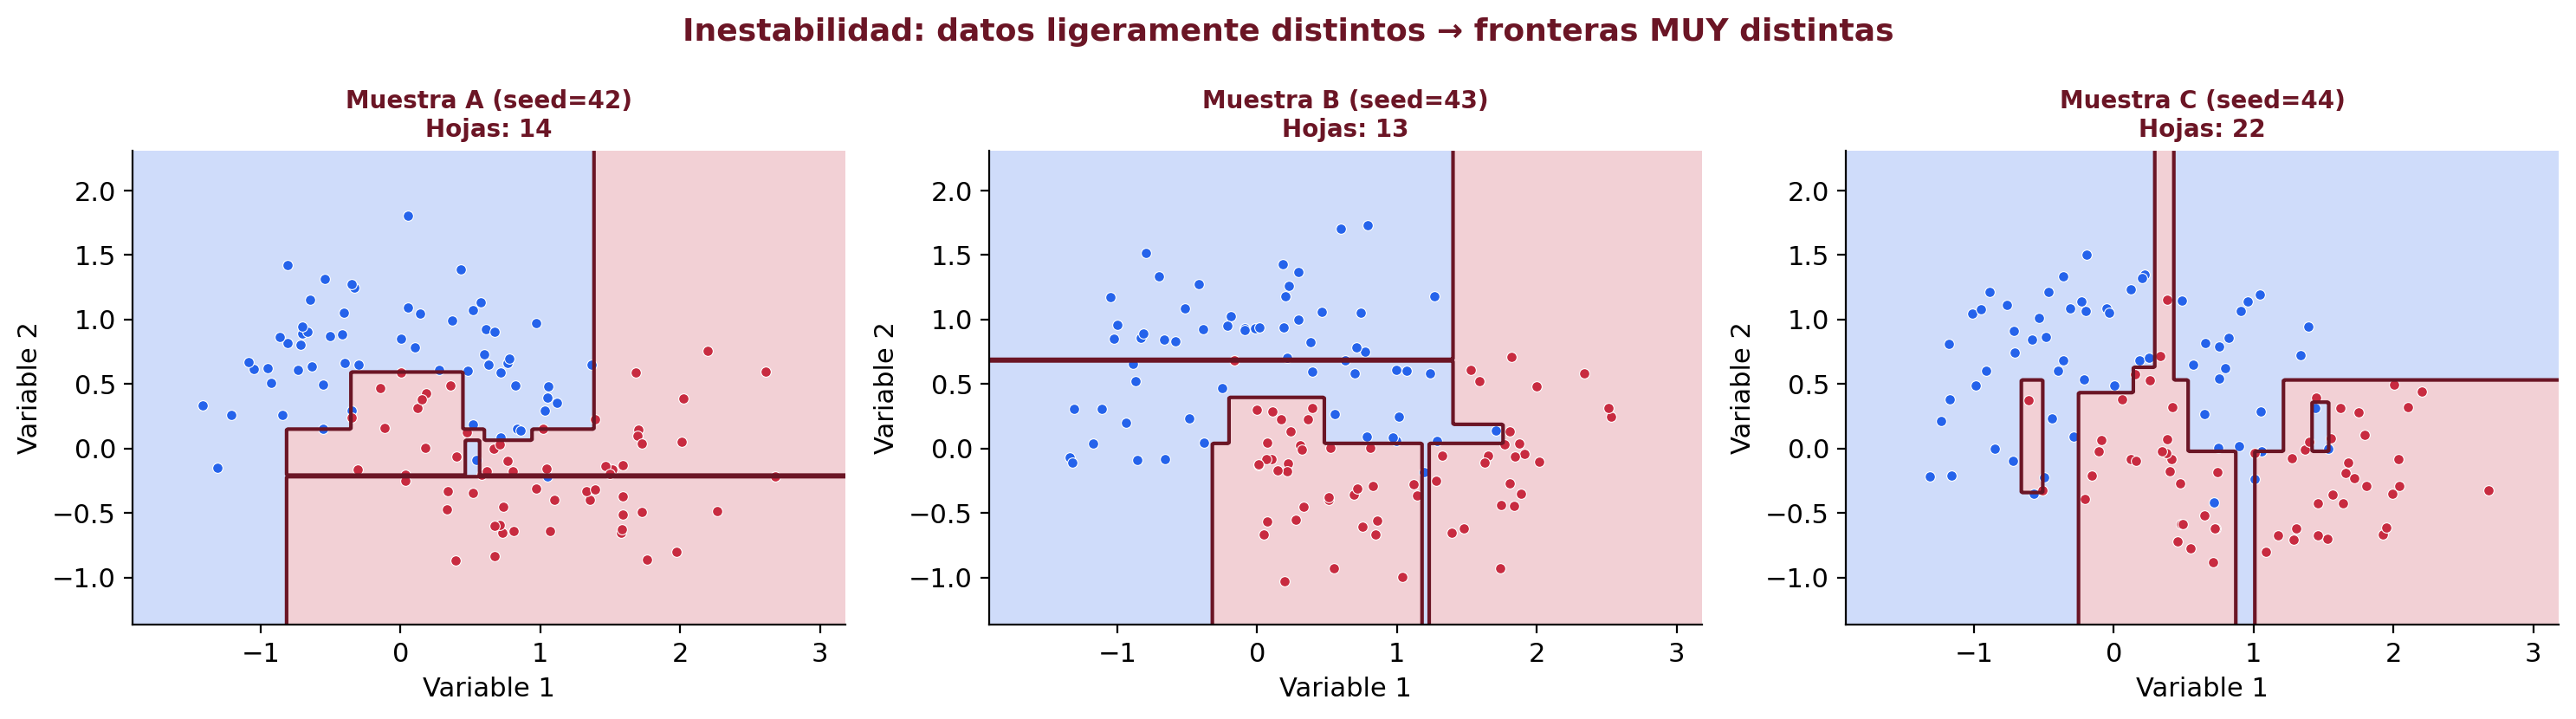
\includegraphics[width=0.95\textwidth]{fig_inestabilidad.png}
  \end{center}

  \vspace{-2pt}
  {\scriptsize\color{textMuted}
    \faLightbulb\hspace{4pt} \textbf{Mismo proceso}, misma distribución,
    misma cantidad de datos. Solo cambia la muestra (como tomar otra
    encuesta del mismo universo). Las fronteras son \textbf{completamente
    distintas}. Eso es inestabilidad.}
\end{frame}

\begin{frame}{¿Por Qué Es Tan Inestable?}
  \vspace{-4pt}
  {\footnotesize\color{arcaDark}\bfseries
    El problema está en cómo funciona el algoritmo:}

  \vspace{6pt}
  {\footnotesize
  \begin{itemize}\setlength{\itemsep}{5pt}
    \item[{\color{arcaRed}\scriptsize\faArrowRight}]
      El primer corte (la raíz) se elige por una diferencia mínima de Gini.
    \item[{\color{arcaRed}\scriptsize\faArrowRight}]
      Si quitas un dato, \textbf{otro corte puede ganar por centésimas}
      $\to$ la raíz cambia.
    \item[{\color{arcaRed}\scriptsize\faArrowRight}]
      Si la raíz cambia, \textbf{todo el resto del árbol cambia}
      (efecto cascada).
    \item[{\color{arcaRed}\scriptsize\faArrowRight}]
      La logística es estable: quitar un dato mueve los coeficientes
      un poquito. El árbol cambia \textit{de forma}.
  \end{itemize}
  }

  \vspace{6pt}
  \begin{tcolorbox}[colback=codeGreen!8, colframe=codeGreen, boxrule=0.5pt, arc=2pt,
    left=6pt, right=6pt, top=4pt, bottom=4pt]
    {\scriptsize\color{arcaDark}
    \faLightbulb\hspace{4pt}\textbf{La solución:} si un árbol es inestable,
    ¿qué pasa si entrenamos \textbf{muchos árboles} con datos ligeramente
    distintos y los hacemos \textbf{votar}? Los errores individuales
    se cancelan. Eso es \textbf{Random Forest}.}
  \end{tcolorbox}
\end{frame}

% =============================================================================
%  BLOQUE C: RANDOM FOREST — INTUICIÓN
% =============================================================================
\sectionframe{Random Forest}{La sabiduría de las multitudes}

\begin{frame}{La Idea: Democracia de Árboles}
  \vspace{-4pt}
  {\footnotesize\color{arcaDark}\bfseries
    Imaginen que quieren saber el peso de un buey en una feria.
    Le preguntan a 100 personas --- individualmente se equivocan,
    pero el \textbf{promedio} es sorprendentemente preciso.}

  \vspace{8pt}
  {\footnotesize
  \begin{itemize}\setlength{\itemsep}{5pt}
    \item[{\color{arcaRed}\scriptsize\faArrowRight}]
      \textbf{Un árbol}: un experto que puede equivocarse mucho.
    \item[{\color{codeGreen}\scriptsize\faArrowRight}]
      \textbf{Random Forest}: 100--500 árboles que \textbf{votan}.
      La mayoría gana.
    \item[{\color{codeGreen}\scriptsize\faArrowRight}]
      Cada árbol se equivoca en cosas \textbf{distintas}. Al votar,
      los errores se cancelan y la predicción es más estable.
  \end{itemize}
  }

  \vspace{6pt}
  \begin{tcolorbox}[colback=arcaGray, colframe=arcaRed, boxrule=0.5pt, arc=2pt,
    left=6pt, right=6pt, top=4pt, bottom=4pt]
    {\scriptsize\color{arcaDark}
    \faKey\hspace{4pt}\textbf{Para que funcione}, los árboles deben ser
    \textbf{diferentes} entre sí. Si todos son iguales, votar no agrega
    nada. Random Forest los hace diferentes con dos trucos: \textbf{bagging}
    y \textbf{features aleatorios}.}
  \end{tcolorbox}
\end{frame}

\begin{frame}{Truco 1: Bagging (Bootstrap Aggregating)}
  \vspace{-4pt}
  {\footnotesize\color{arcaDark}\bfseries
    Cada árbol se entrena con una \textbf{muestra distinta} de los datos.}

  \vspace{6pt}
  {\footnotesize
  \begin{itemize}\setlength{\itemsep}{5pt}
    \item[{\color{arcaRed}\scriptsize\faArrowRight}]
      Del dataset original (N filas), tomar N filas \textbf{al azar
      con reemplazo} (bootstrap). Algunas filas se repiten, otras quedan fuera.
    \item[{\color{arcaRed}\scriptsize\faArrowRight}]
      Entrenar un árbol con esa muestra.
    \item[{\color{arcaRed}\scriptsize\faArrowRight}]
      Repetir 100, 200 o 500 veces $\to$ 100, 200 o 500 árboles distintos.
    \item[{\color{arcaRed}\scriptsize\faArrowRight}]
      Para predecir: cada árbol vota $\to$ la clase con más votos gana.
  \end{itemize}
  }

  \vspace{6pt}
  {\scriptsize\color{textMuted}
    \faLightbulb\hspace{4pt} ``Con reemplazo'' = un paciente puede
    aparecer 2 veces en una muestra y 0 veces en otra. Así cada árbol
    ve una \textit{perspectiva distinta} de los datos.}
\end{frame}

\begin{frame}{Truco 2: Features Aleatorios (\texttt{max\_features})}
  \vspace{-4pt}
  {\footnotesize\color{arcaDark}\bfseries
    Además de datos distintos, cada corte solo considera un
    \textbf{subconjunto aleatorio} de variables.}

  \vspace{6pt}
  {\footnotesize
  \begin{itemize}\setlength{\itemsep}{5pt}
    \item[{\color{arcaRed}\scriptsize\faArrowRight}]
      Si tenemos 15 variables, en cada nodo el árbol solo puede
      elegir entre \textbf{4 variables al azar} (por defecto $\sqrt{15} \approx 4$).
    \item[{\color{arcaRed}\scriptsize\faArrowRight}]
      Esto evita que todos los árboles pongan ``edad'' en la raíz.
    \item[{\color{arcaRed}\scriptsize\faArrowRight}]
      Algunos árboles empiezan con glucosa, otros con BMI, otros con
      tabaquismo $\to$ son genuinamente \textbf{diferentes}.
  \end{itemize}
  }

  \vspace{6pt}
  \begin{tcolorbox}[colback=codeGreen!8, colframe=codeGreen, boxrule=0.5pt, arc=2pt,
    left=6pt, right=6pt, top=4pt, bottom=4pt]
    {\scriptsize\color{arcaDark}
    \faCheckCircle\hspace{4pt}\textbf{Resultado:} datos distintos +
    variables distintas = árboles genuinamente distintos.
    El voto de la mayoría produce una predicción \textbf{estable y precisa}.}
  \end{tcolorbox}
\end{frame}

\begin{frame}[shrink=22]{Bagging Visual: Cada Árbol Ve Datos Distintos}
  \vspace{-4pt}
  \begin{center}
    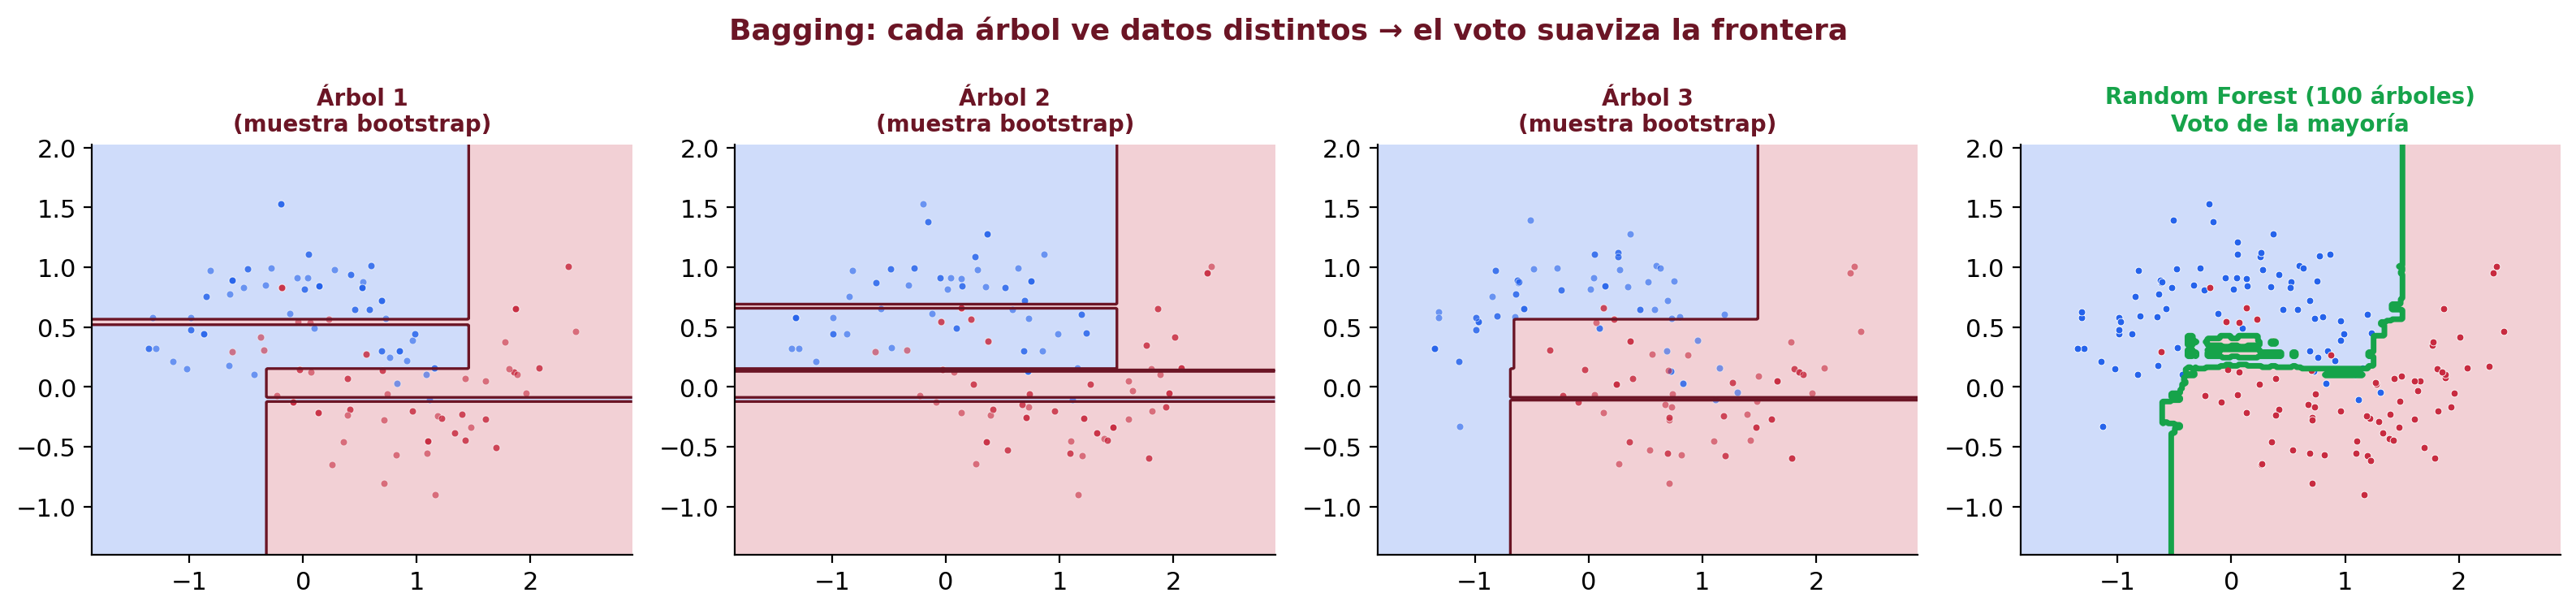
\includegraphics[width=0.95\textwidth]{fig_bagging.png}
  \end{center}

  \vspace{-2pt}
  {\scriptsize\color{textMuted}
    \faLightbulb\hspace{4pt} Cada árbol tiene una frontera \textbf{distinta}
    (y un poco ruidosa). Pero al votar los 100, la frontera final
    (derecha, en verde) es \textbf{suave y estable}.}
\end{frame}

\begin{frame}[shrink=15]{1 Árbol vs Random Forest: La Diferencia}
  \vspace{-4pt}
  \begin{center}
    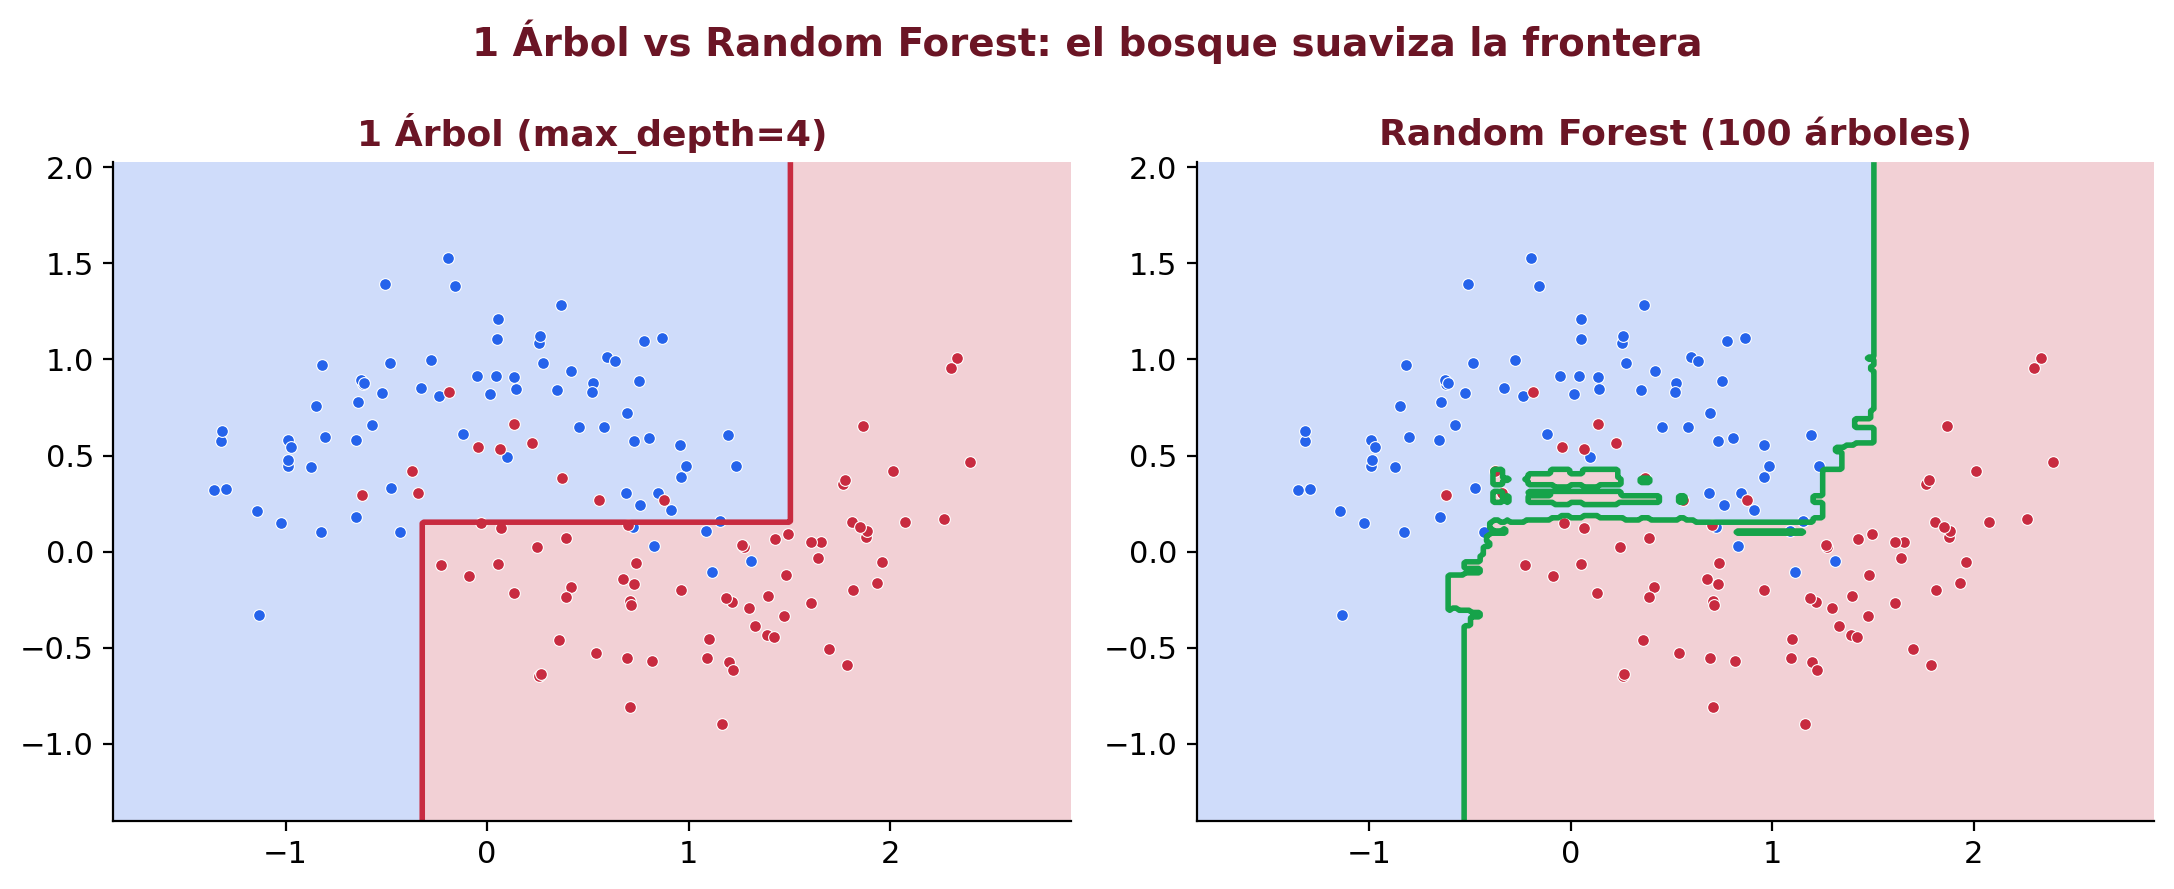
\includegraphics[width=0.88\textwidth]{fig_arbol_vs_rf.png}
  \end{center}

  \vspace{-2pt}
  {\scriptsize\color{textMuted}
    \faLightbulb\hspace{4pt} El árbol individual tiene una frontera
    \textbf{dentada} (sobreajustada). El Random Forest la \textbf{suaviza}
    porque promedia muchos árboles imperfectos.}
\end{frame}

% =============================================================================
%  BLOQUE D: RANDOMFORESTCLASSIFIER
% =============================================================================
\sectionframe{RandomForestClassifier}{De la teoría al código}

\begin{frame}[fragile,shrink=18]{Tu Primer Random Forest --- 5 Líneas}
  \vspace{-6pt}
  \begin{pyblock}
from sklearn.ensemble import RandomForestClassifier

rf = RandomForestClassifier(
    n_estimators=200,          # 200 arboles
    max_depth=8,               # cada arbol podado a 8
    class_weight="balanced",   # desbalance
    random_state=42)
rf.fit(X_train, y_train)

print(f"Accuracy train: {rf.score(X_train, y_train):.3f}")
print(f"Accuracy test:  {rf.score(X_test, y_test):.3f}")
  \end{pyblock}

  \vspace{4pt}
  {\scriptsize\color{arcaDark}
    \faArrowRight\hspace{4pt} Noten que \textbf{no necesita escalado}
    (igual que el árbol). Y usa \texttt{class\_weight="balanced"}
    para el desbalance (igual que logística y árbol).}
\end{frame}

\begin{frame}[shrink=5]{Hiperparámetros del Random Forest}
  \vspace{-4pt}
  {\footnotesize\color{arcaDark}\bfseries
    Los más importantes --- en orden de prioridad:}

  \vspace{6pt}
  {\scriptsize
  \begin{tabular}{@{}lp{5.5cm}p{4cm}@{}}
    \toprule
    \textbf{Parámetro} & \textbf{Qué controla} & \textbf{Valor sugerido} \\
    \midrule
    \texttt{n\_estimators} & Cuántos árboles entrenar. Más = mejor pero más lento. & 100--500 (rendimiento decreciente). \\
    \texttt{max\_depth} & Profundidad máxima de cada árbol. & 5--15 (o \texttt{None}). \\
    \texttt{max\_features} & Variables por corte. & \texttt{"sqrt"} (default, bueno). \\
    \texttt{min\_samples\_leaf} & Mín. muestras en cada hoja. & 5--20. \\
    \texttt{class\_weight} & Manejo del desbalance. & \texttt{"balanced"}. \\
    \bottomrule
  \end{tabular}
  }

  \vspace{6pt}
  \begin{tcolorbox}[colback=codeGreen!8, colframe=codeGreen, boxrule=0.5pt, arc=2pt,
    left=6pt, right=6pt, top=4pt, bottom=4pt]
    {\scriptsize\color{arcaDark}
    \faLightbulb\hspace{4pt}\textbf{Buena noticia:} Random Forest funciona
    bien ``de fábrica''. Con los defaults de sklearn ya supera a la mayoría
    de modelos simples. Ajustar hiperparámetros ayuda, pero no es urgente.}
  \end{tcolorbox}
\end{frame}

\begin{frame}[shrink=15]{¿Cuántos Árboles Necesito?}
  \vspace{-4pt}
  \begin{center}
    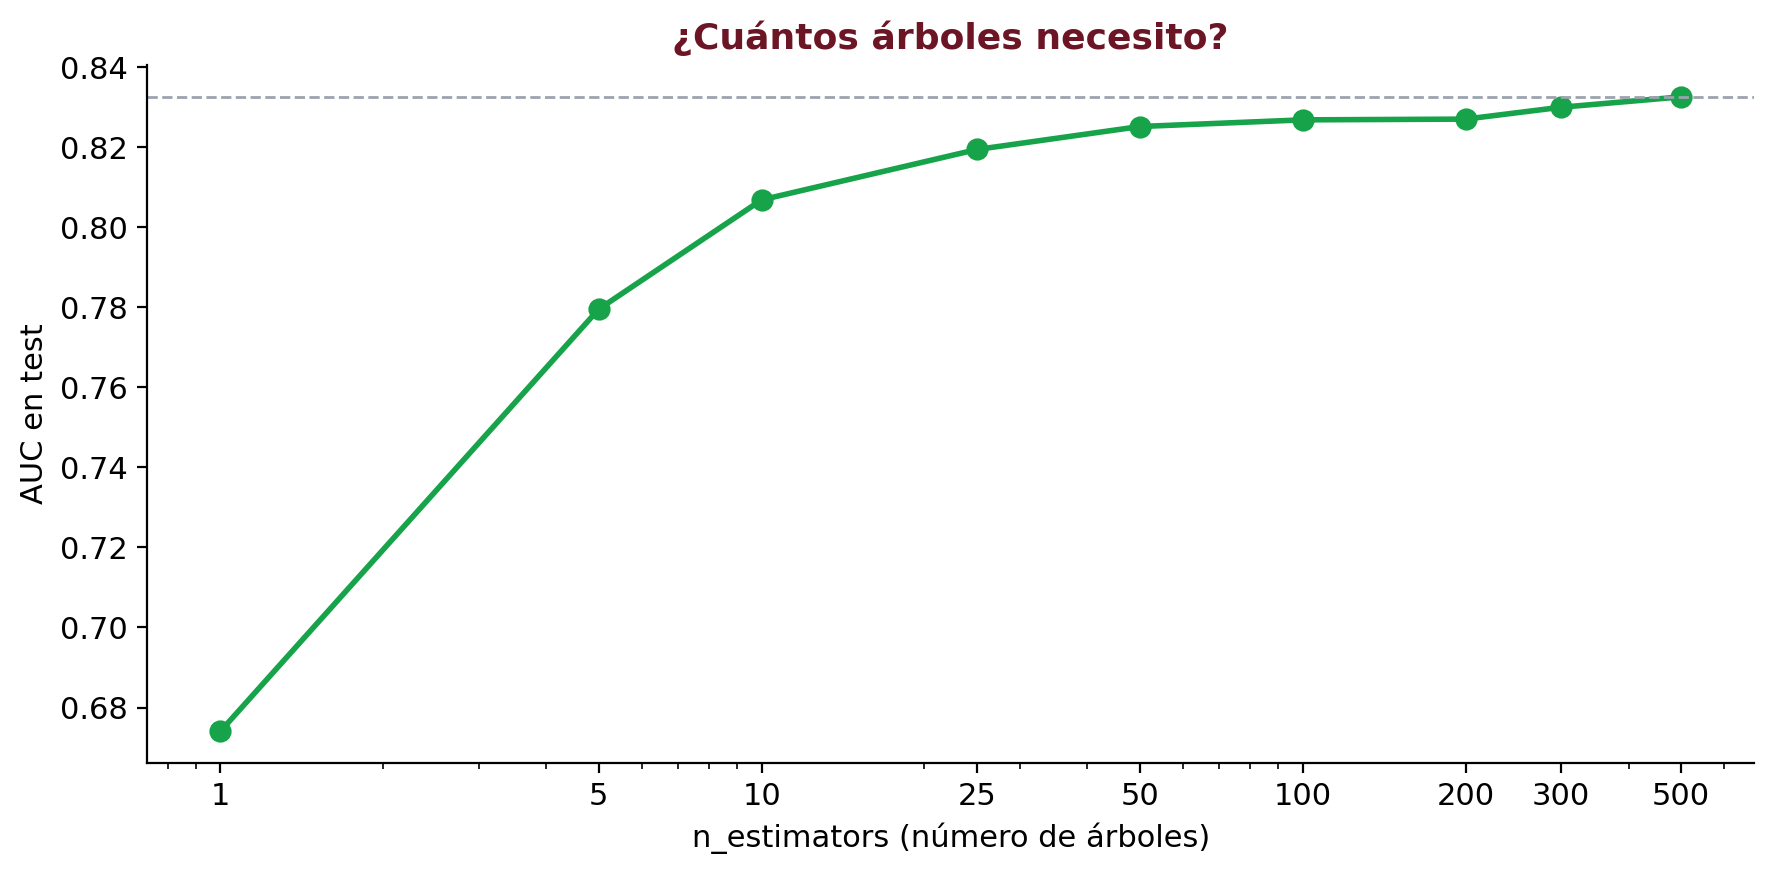
\includegraphics[width=0.8\textwidth]{fig_n_estimators.png}
  \end{center}

  \vspace{-2pt}
  {\scriptsize\color{textMuted}
    \faLightbulb\hspace{4pt} \textbf{Rendimiento decreciente:} de 1 a 50
    árboles la mejora es enorme. De 100 a 500, marginal. En la práctica,
    100--200 es suficiente. No vale la pena esperar por 1000.}
\end{frame}

\begin{frame}[fragile,shrink=18]{Feature Importance en Random Forest}
  \vspace{-6pt}
  \begin{pyblock}
importancias = pd.DataFrame({
    "feature": X_train.columns,
    "importancia": rf.feature_importances_
}).sort_values("importancia", ascending=True).tail(10)

fig = px.bar(importancias, x="importancia", y="feature",
             orientation="h",
             title="Top 10 variables (Random Forest)")
fig.show()
  \end{pyblock}

  \vspace{4pt}
  {\scriptsize\color{arcaDark}
    \faKey\hspace{4pt} La importancia del RF es más \textbf{estable} que la
    del árbol individual, porque promedia la importancia de 200 árboles.
    Es más confiable.}
\end{frame}

\begin{frame}[shrink=15]{Importancia: 1 Árbol vs Random Forest}
  \vspace{-4pt}
  \begin{center}
    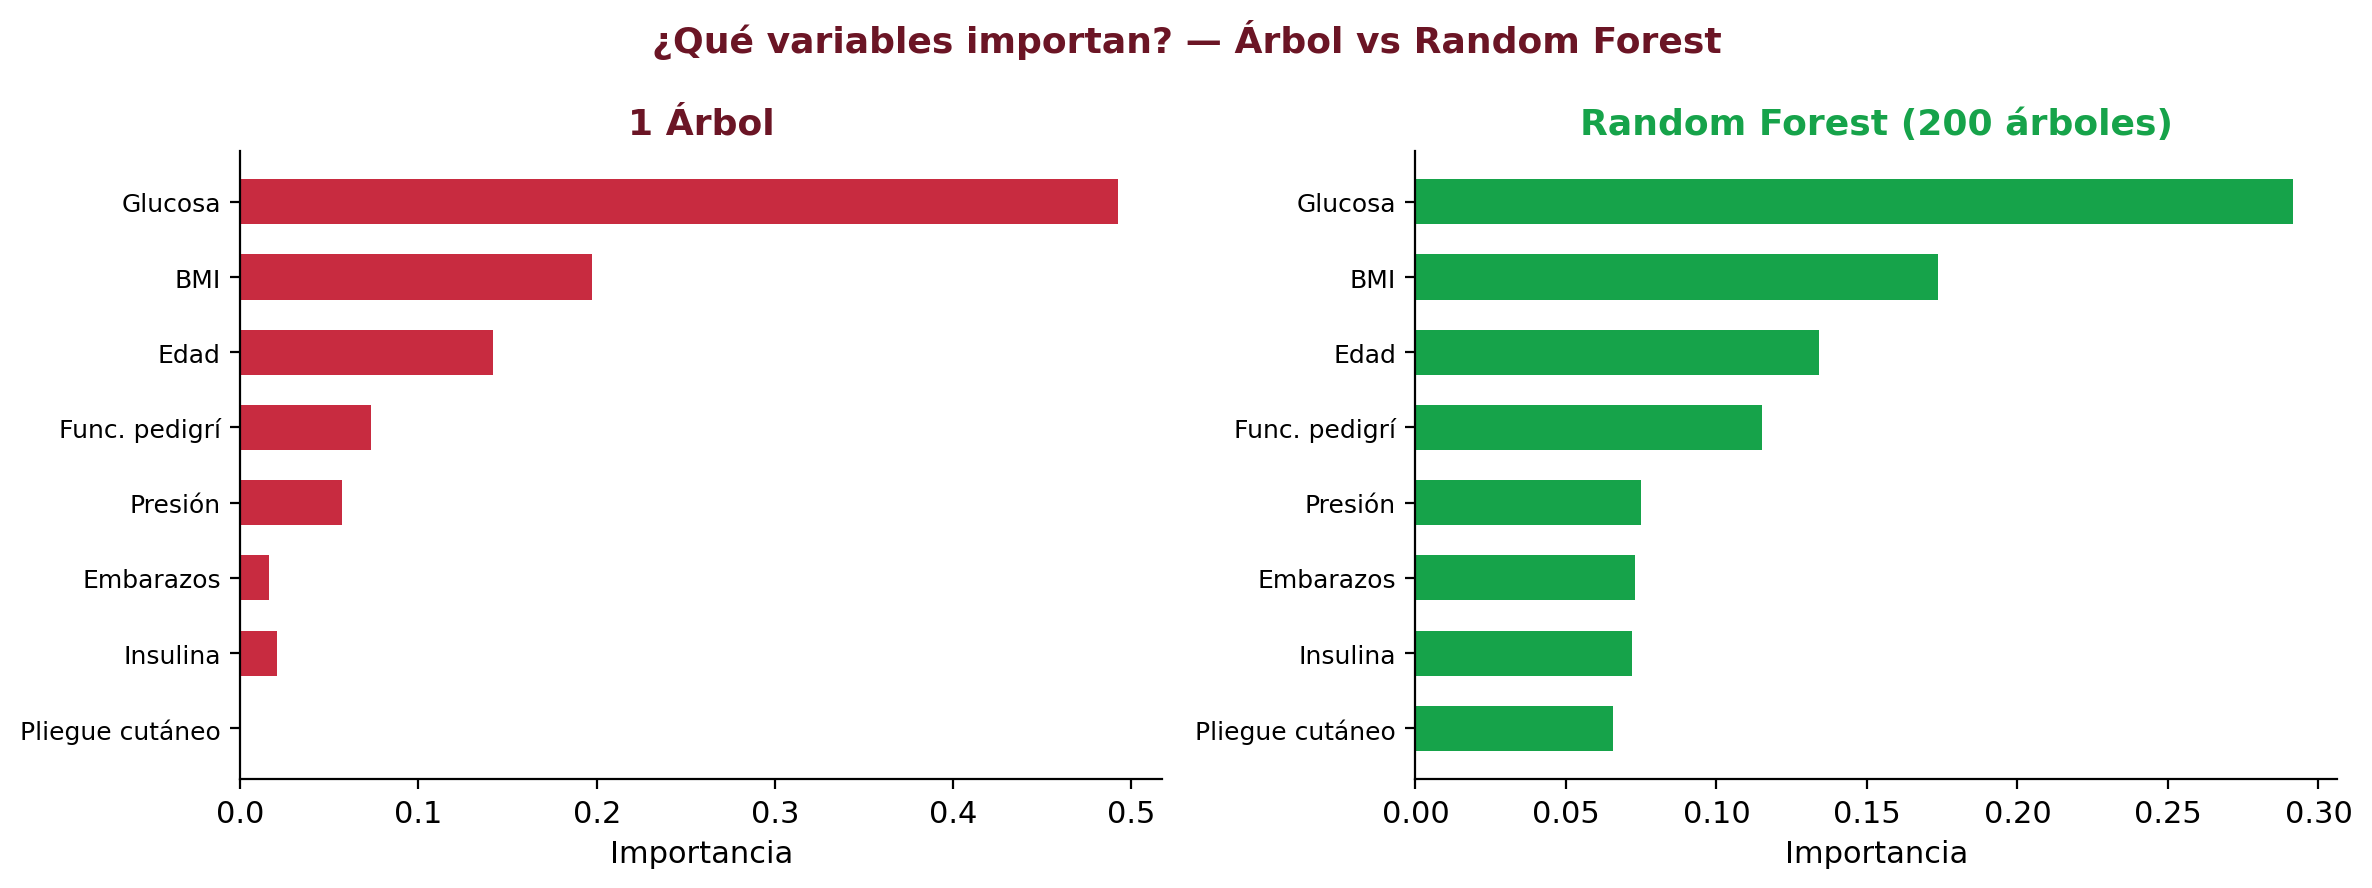
\includegraphics[width=0.88\textwidth]{fig_importances_rf.png}
  \end{center}

  \vspace{-2pt}
  {\scriptsize\color{textMuted}
    \faLightbulb\hspace{4pt} El árbol individual puede dar importancia 0
    a variables útiles (si otra correlacionada ``ganó''). El RF distribuye
    la importancia de forma más \textbf{justa} porque cada árbol usa
    subconjuntos distintos de variables.}
\end{frame}

\begin{frame}[shrink=5]{Ejercicio 1: Tu Primer Random Forest}
  \vspace{-4pt}
  {\footnotesize\color{arcaDark}\bfseries
    \faClock\hspace{4pt} 12 minutos --- en el notebook:}

  \vspace{6pt}
  {\footnotesize
  \begin{enumerate}\setlength{\itemsep}{4pt}
    \item Entrenen un RF con \texttt{n\_estimators=200}, \texttt{max\_depth=8},
      \texttt{class\_weight="balanced"}.
    \item Reporten accuracy, recall, AUC y AP en test.
    \item Grafiquen el top 10 de \texttt{feature\_importances\_}.
    \item Hagan el barrido de \texttt{n\_estimators} (1, 10, 50, 100, 200, 500)
      y grafiquen AUC vs número de árboles.
    \item ¿Cuántos árboles son ``suficientes''?
  \end{enumerate}
  }
\end{frame}

% =============================================================================
%  BLOQUE E: COMPARACIÓN TRIPLE
% =============================================================================
\sectionframe{Comparación Triple}{Logística vs Árbol vs Random Forest}

\begin{frame}[fragile,shrink=25]{Los 3 Modelos en las Mismas Métricas}
  \vspace{-6pt}
  \begin{pyblock}
from sklearn.metrics import classification_report, roc_auc_score

modelos = {
    "Logistica": (modelo_lr, X_test_s),
    "Arbol":     (arbol, X_test),
    "RF":        (rf, X_test),
}
for nombre, (mod, X_t) in modelos.items():
    y_pred = mod.predict(X_t)
    y_prob = mod.predict_proba(X_t)[:, 1]
    print(f"=== {nombre} ===")
    print(f"AUC: {roc_auc_score(y_test, y_prob):.3f}  "
          f"AP: {average_precision_score(y_test, y_prob):.3f}")
    print(classification_report(y_test, y_pred,
          target_names=["No Diabetes","Diabetes"]))
  \end{pyblock}
\end{frame}

\begin{frame}[fragile,shrink=18]{3 Curvas ROC en un Solo Gráfico}
  \vspace{-6pt}
  \begin{pyblock}
fig = go.Figure()
for nombre, (mod, X_t), color in zip(
    ["Logistica","Arbol","Random Forest"],
    modelos.values(),
    ["#2563EB","#C82B40","#16A34A"]):
    y_prob = mod.predict_proba(X_t)[:, 1]
    fpr, tpr, _ = roc_curve(y_test, y_prob)
    auc = roc_auc_score(y_test, y_prob)
    fig.add_trace(go.Scatter(x=fpr, y=tpr, mode="lines",
        name=f"{nombre} (AUC={auc:.3f})",
        line=dict(color=color)))
fig.add_shape(type="line", line=dict(dash="dash"),
              x0=0,x1=1,y0=0,y1=1)
fig.update_layout(title="ROC: Logistica vs Arbol vs RF",
    xaxis_title="FPR", yaxis_title="TPR")
fig.show()
  \end{pyblock}
\end{frame}

\begin{frame}[shrink=15]{AUC por Modelo (CV) --- Diabetes}
  \vspace{-4pt}
  \begin{center}
    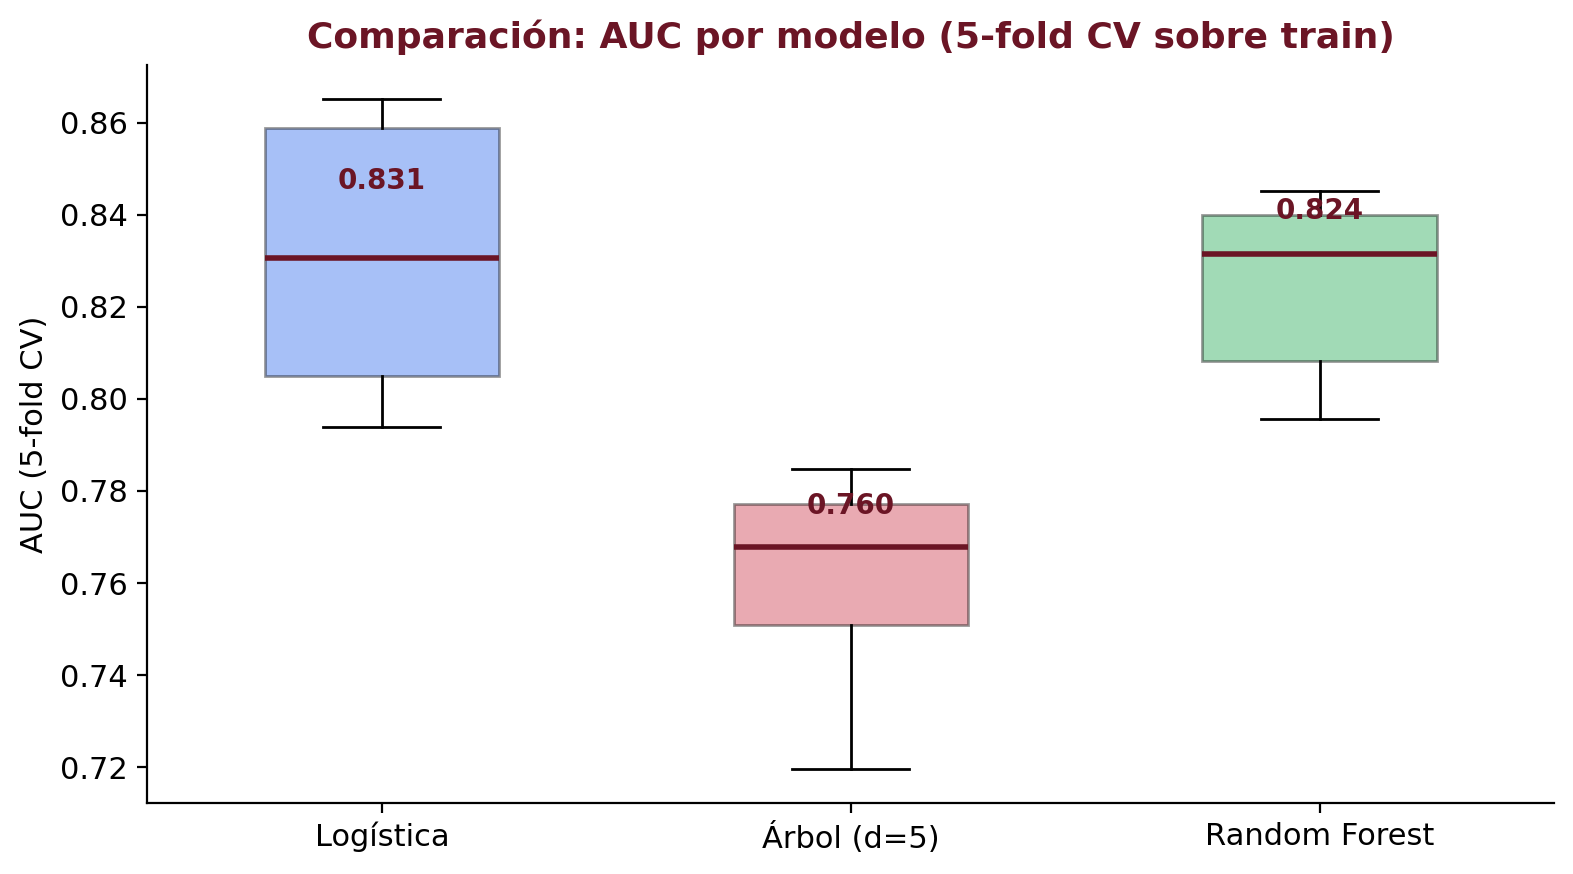
\includegraphics[width=0.75\textwidth]{fig_comparacion_cv.png}
  \end{center}

  \vspace{-2pt}
  {\scriptsize\color{textMuted}
    \faLightbulb\hspace{4pt} Cada caja muestra la distribución de AUC
    en los 5 folds de CV. El Random Forest tiene el \textbf{promedio más alto}
    y la \textbf{menor variabilidad}. En diabetes, la diferencia con
    logística es más clara que en stroke.}
\end{frame}

\begin{frame}[shrink=5]{Ejercicio 2: Comparación Triple}
  \vspace{-4pt}
  {\footnotesize\color{arcaDark}\bfseries
    \faClock\hspace{4pt} 10 minutos --- en el notebook:}

  \vspace{6pt}
  {\footnotesize
  \begin{enumerate}\setlength{\itemsep}{4pt}
    \item Grafiquen las 3 curvas ROC en un gráfico.
    \item Grafiquen las 3 curvas PR en otro gráfico.
    \item ¿Cuál modelo tiene mejor AUC? ¿Y mejor AP?
    \item ¿Cuál modelo elegirían para producción y por qué?
    \item Si el médico pide \textbf{explicar} por qué marcaron a un
      paciente, ¿cuál modelo les facilita eso?
  \end{enumerate}
  }
\end{frame}

% =============================================================================
%  BLOQUE F: PARÁMETROS, HIPERPARÁMETROS Y VALIDACIÓN CRUZADA
% =============================================================================
\sectionframe{Hiperparámetros y Validación Cruzada}{Afinar el modelo con rigor}

\begin{frame}{Parámetros vs Hiperparámetros}
  \vspace{-4pt}
  {\footnotesize\color{arcaDark}\bfseries
    Dos conceptos que debemos distinguir:}

  \vspace{6pt}
  {\scriptsize
  \begin{tabular}{@{}p{3cm}p{5cm}p{4.5cm}@{}}
    \toprule
     & \textbf{\color{codeBlue}Parámetros} & \textbf{\color{arcaRed}Hiperparámetros} \\
    \midrule
    \textbf{¿Quién los define?} & El \textbf{algoritmo}, durante \texttt{.fit()}. & \textbf{Nosotros}, antes de \texttt{.fit()}. \\
    \textbf{Ejemplos en logística} & Coeficientes $\beta_0, \beta_1\ldots$ & \texttt{C}, \texttt{max\_iter}. \\
    \textbf{Ejemplos en RF} & Los cortes internos de cada árbol. & \texttt{n\_estimators}, \texttt{max\_depth}. \\
    \textbf{¿Se pueden optimizar?} & El algoritmo los optimiza automáticamente. & Nosotros debemos buscar los mejores. \\
    \bottomrule
  \end{tabular}
  }

  \vspace{6pt}
  \begin{tcolorbox}[colback=arcaGray, colframe=arcaRed, boxrule=0.5pt, arc=2pt,
    left=6pt, right=6pt, top=4pt, bottom=4pt]
    {\scriptsize\color{arcaDark}
    \faKey\hspace{4pt}\textbf{Hyperparameter tuning} = encontrar la
    combinación de hiperparámetros que produce el mejor rendimiento.
    El problema: ¿con qué datos medimos ``mejor rendimiento''?}
  \end{tcolorbox}
\end{frame}

\begin{frame}{¿Por Qué No Podemos Usar Test para Elegir Hiperparámetros?}
  \vspace{-4pt}
  {\footnotesize\color{arcaDark}\bfseries
    En clase 17 probamos \texttt{max\_depth} = 1 a 20 y elegimos el que
    diera mejor accuracy en \textbf{test}. Eso tiene un problema sutil.}

  \vspace{6pt}
  {\footnotesize
  \begin{itemize}\setlength{\itemsep}{5pt}
    \item[{\color{arcaRed}\scriptsize\faArrowRight}]
      Cada modelo (depth=1, depth=2, \ldots) sí evalúa en datos que
      \textbf{no vio durante su entrenamiento}. Eso está bien.
    \item[{\color{arcaRed}\scriptsize\faArrowRight}]
      El problema es la \textbf{selección}: de 20 opciones, elegimos la que
      tuvo mejor score en \textbf{este test particular}. Parte de ese score
      es skill real del modelo, pero parte es \textbf{suerte} --- coincidencias
      entre los hiperparámetros y las particularidades de ese split.
    \item[{\color{arcaRed}\scriptsize\faArrowRight}]
      Si hiciéramos otro split, el ``mejor'' depth podría ser distinto.
      Estamos \textbf{sobreajustando los hiperparámetros al test}.
    \item[{\color{codeGreen}\scriptsize\faArrowRight}]
      \textbf{Solución:} necesitamos datos que el modelo no vea durante
      el entrenamiento \textbf{ni} durante la selección de hiperparámetros.
  \end{itemize}
  }
\end{frame}

\begin{frame}{Train / Validación / Test --- Los Tres Roles}
  \vspace{-4pt}
  {\footnotesize\color{arcaDark}\bfseries
    El flujo correcto separa los datos en tres funciones:}

  \vspace{6pt}
  {\scriptsize
  \begin{tabular}{@{}p{2.5cm}p{4.5cm}p{5cm}@{}}
    \toprule
    \textbf{Conjunto} & \textbf{Para qué se usa} & \textbf{Cuántas veces} \\
    \midrule
    \textbf{\color{codeBlue}Train} & El modelo aprende de estos datos (\texttt{.fit()}). & Muchas veces. \\
    \textbf{\color{codeOrange}Validación} & Comparar hiperparámetros y elegir los mejores. & Muchas veces. \\
    \textbf{\color{arcaRed}Test} & Evaluar el modelo \textbf{final} y reportar la métrica definitiva. & \textbf{Una sola vez.} \\
    \bottomrule
  \end{tabular}
  }

  \vspace{6pt}
  \begin{tcolorbox}[colback=arcaRed!8, colframe=arcaRed, boxrule=0.5pt, arc=2pt,
    left=6pt, right=6pt, top=4pt, bottom=4pt]
    {\scriptsize\color{arcaDark}
    \faExclamationTriangle\hspace{4pt} Partir en 3 conjuntos desperdicia datos.
    Con 5110 filas, cada conjunto queda chico.
    \textbf{Validación cruzada} resuelve esto: usa el train como
    train Y validación simultáneamente, sin desperdiciar nada.}
  \end{tcolorbox}
\end{frame}

% =============================================================================
%  BLOQUE G: VALIDACIÓN CRUZADA
% =============================================================================
\sectionframe{Validación Cruzada}{Evaluar sin desperdiciar datos}

\begin{frame}{K-Fold Cross-Validation}
  \vspace{-4pt}
  {\footnotesize\color{arcaDark}\bfseries
    Se divide el conjunto de train en $K$ bloques iguales (folds).
    En cada iteración, un bloque distinto sirve como validación:}

  \vspace{4pt}
  {\footnotesize
  \begin{enumerate}\setlength{\itemsep}{3pt}
    \item Dividir train en $K$ bloques (típicamente $K=5$ o $K=10$).
    \item Para $i = 1, 2, \ldots, K$:
      \begin{itemize}
        \item Entrenar con los $K-1$ bloques restantes.
        \item Evaluar con el bloque $i$.
        \item Guardar el score.
      \end{itemize}
    \item Reportar el \textbf{promedio} y la \textbf{desviación estándar}
      de los $K$ scores.
  \end{enumerate}
  }

  \vspace{4pt}
  {\scriptsize\color{textMuted}
    \faArrowRight\hspace{4pt} Cada observación es validación
    \textbf{exactamente una vez}. No se desperdicia nada.
    El promedio es más confiable que un solo split.}
\end{frame}

\begin{frame}[shrink=18]{K-Fold --- Diagrama}
  \vspace{-4pt}
  \begin{center}
    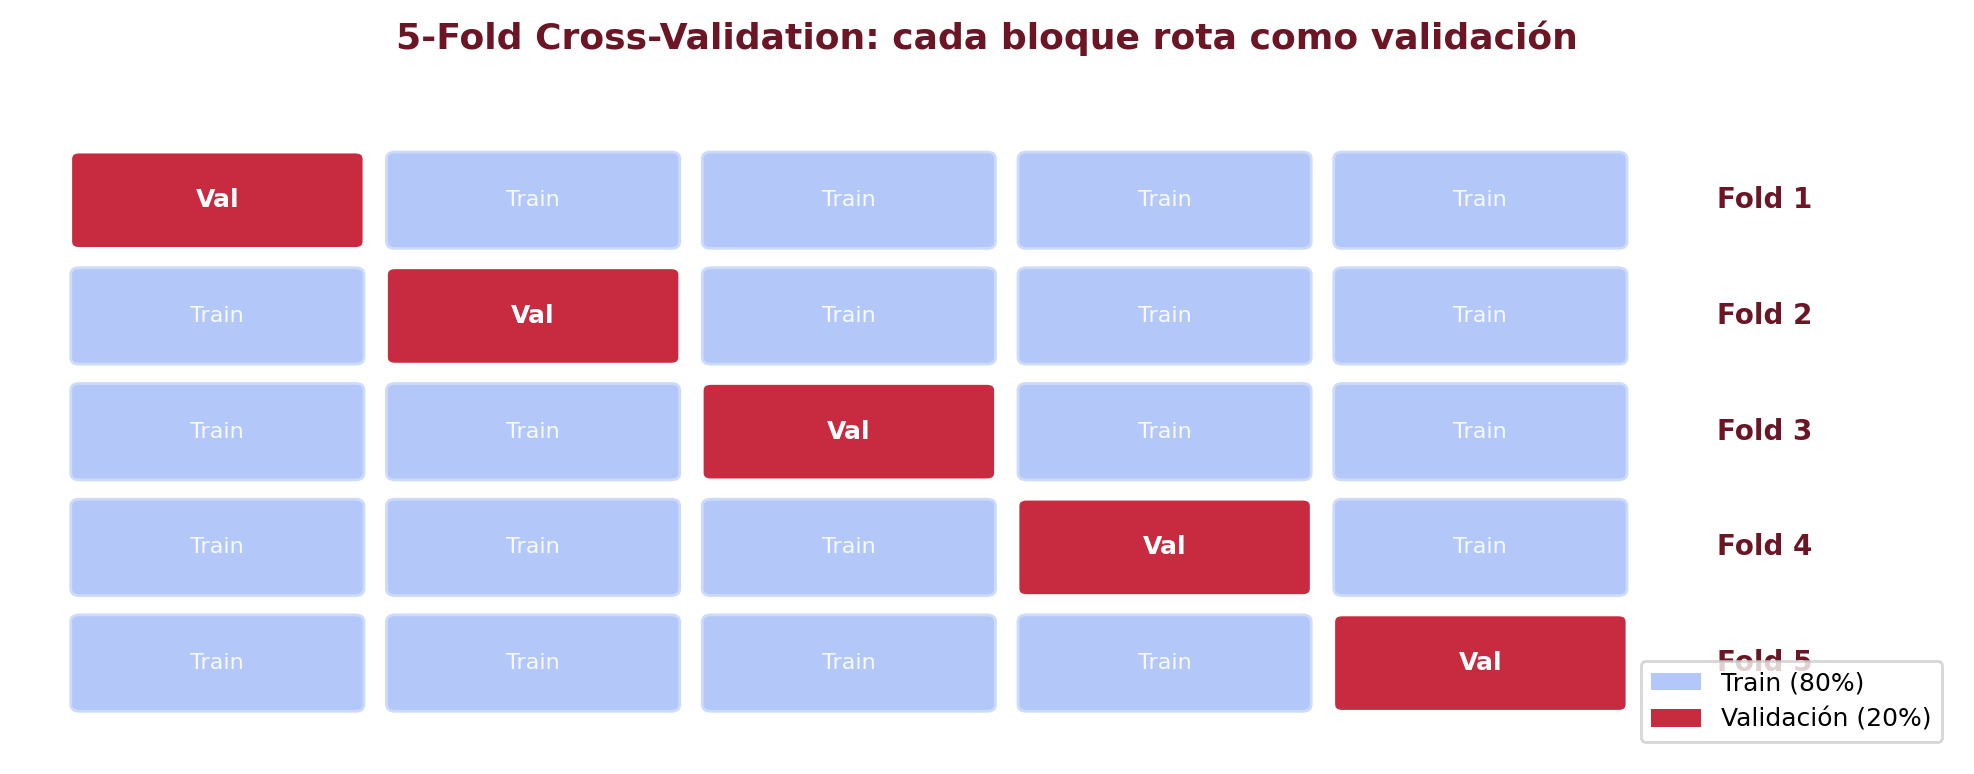
\includegraphics[width=0.85\textwidth]{fig_cv.png}
  \end{center}

  \vspace{-2pt}
  {\scriptsize\color{textMuted}
    \faLightbulb\hspace{4pt} En cada fold, el bloque rojo es validación
    y el resto es entrenamiento. Al terminar los 5 folds, cada dato
    fue validación exactamente una vez.
    El \textbf{promedio} de los 5 scores es la estimación de rendimiento.}
\end{frame}

\begin{frame}[fragile,shrink=18]{Código: \texttt{cross\_val\_score}}
  \vspace{-6pt}
  \begin{pyblock}
from sklearn.model_selection import cross_val_score

# 5-fold CV sobre el Random Forest
scores = cross_val_score(rf, X_train, y_train,
                         cv=5, scoring="roc_auc")

print(f"AUC por fold: {scores.round(3)}")
print(f"AUC promedio: {scores.mean():.3f} +/- {scores.std():.3f}")
  \end{pyblock}

  \vspace{4pt}
  \begin{outputblock}
AUC por fold: [0.82  0.79  0.85  0.81  0.83]
AUC promedio: 0.820 +/- 0.020
  \end{outputblock}

  \vspace{4pt}
  {\scriptsize\color{arcaDark}
  \begin{itemize}\setlength{\itemsep}{3pt}
    \item[{\color{arcaRed}\scriptsize\faArrowRight}]
      \texttt{cv=5}: 5 particiones. Valores comunes: 5 o 10.
    \item[{\color{arcaRed}\scriptsize\faArrowRight}]
      \texttt{scoring="roc\_auc"}: métrica a evaluar (también
      \texttt{"recall"}, \texttt{"precision"}, \texttt{"f1"}).
    \item[{\color{arcaRed}\scriptsize\faArrowRight}]
      El \textbf{$\pm$ 0.020} dice que el AUC varía poco entre folds
      $\to$ el modelo es \textbf{estable}.
  \end{itemize}
  }
\end{frame}

\begin{frame}{¿Cómo Sé Qué Hiperparámetros Tiene un Modelo?}
  \vspace{-4pt}
  {\footnotesize\color{arcaDark}\bfseries
    Cada modelo de sklearn tiene hiperparámetros distintos.
    La forma de saberlos: \textbf{leer la documentación}.}

  \vspace{6pt}
  {\scriptsize
  \begin{tabular}{@{}lp{8cm}@{}}
    \toprule
    \textbf{Modelo} & \textbf{Hiperparámetros principales} \\
    \midrule
    \texttt{LogisticRegression} & \texttt{C} (regularización), \texttt{l1\_ratio} (Lasso vs Ridge). \\
    \texttt{DecisionTreeClassifier} & \texttt{max\_depth}, \texttt{min\_samples\_leaf}, \texttt{min\_samples\_split}. \\
    \texttt{RandomForestClassifier} & \texttt{n\_estimators}, \texttt{max\_depth}, \texttt{max\_features}, \texttt{min\_samples\_leaf}. \\
    \bottomrule
  \end{tabular}
  }

  \vspace{6pt}
  {\footnotesize
  \begin{itemize}\setlength{\itemsep}{4pt}
    \item[{\color{arcaRed}\scriptsize\faArrowRight}]
      En Python: \texttt{modelo.get\_params()} muestra todos los
      hiperparámetros con sus valores actuales.
    \item[{\color{arcaRed}\scriptsize\faArrowRight}]
      En la web: \texttt{scikit-learn.org} $\to$ buscar el nombre del modelo
      $\to$ sección ``Parameters''.
    \item[{\color{codeGreen}\scriptsize\faArrowRight}]
      \textbf{No hay que tunear todos.} Empezar con los 2--3 más importantes.
  \end{itemize}
  }
\end{frame}

\begin{frame}{GridSearchCV = Grid Search + Cross-Validation}
  \vspace{-4pt}
  {\footnotesize\color{arcaDark}\bfseries
    El nombre lo dice todo: es una \textbf{búsqueda en grilla} donde
    cada combinación se evalúa con \textbf{cross-validation}.}

  \vspace{6pt}
  {\footnotesize
  \begin{itemize}\setlength{\itemsep}{5pt}
    \item[{\color{arcaRed}\scriptsize\faArrowRight}]
      \textbf{Grid Search}: probar todas las combinaciones posibles de
      hiperparámetros (grilla = tabla de opciones).
    \item[{\color{arcaRed}\scriptsize\faArrowRight}]
      \textbf{CV}: para cada combinación, en vez de evaluar con un solo
      split, hace \textbf{K-Fold cross-validation} y reporta el promedio.
    \item[{\color{arcaRed}\scriptsize\faArrowRight}]
      El parámetro \texttt{cv=5} significa: cada combinación se evalúa
      con 5-fold CV. Si hay 45 combinaciones, son $45 \times 5 = 225$
      entrenamientos.
    \item[{\color{codeGreen}\scriptsize\faArrowRight}]
      Al final, elige la combinación con el \textbf{mejor score promedio}
      en los 5 folds. Luego reentrena con \textbf{todo} el train.
  \end{itemize}
  }
\end{frame}

\begin{frame}[fragile,shrink=22]{Código: GridSearchCV Paso a Paso}
  \vspace{-6pt}
  \begin{pyblock}
from sklearn.model_selection import GridSearchCV

# Paso 1: definir que valores probar para cada hiperparametro
# Las llaves son EXACTAMENTE los nombres de la documentacion
param_grid = {
    "n_estimators": [100, 200, 300],   # 3 opciones
    "max_depth": [3, 5, 8, 12, None],  # 5 opciones (None = sin limite)
    "min_samples_leaf": [1, 5, 10],    # 3 opciones
}
# Total: 3 x 5 x 3 = 45 combinaciones

# Paso 2: crear GridSearchCV
grid = GridSearchCV(
    RandomForestClassifier(class_weight="balanced", random_state=42),
    param_grid,
    cv=5,               # 5-fold cross-validation por combinacion
    scoring="roc_auc",  # metrica para comparar
    n_jobs=-1)           # usar todos los nucleos del CPU

# Paso 3: correr (45 combos x 5 folds = 225 entrenamientos)
grid.fit(X_train, y_train)
  \end{pyblock}
\end{frame}

\begin{frame}[fragile,shrink=10]{Resultados del GridSearchCV}
  \vspace{-4pt}
  \begin{pyblock}
# Mejor combinacion encontrada
print(f"Mejor AUC (CV): {grid.best_score_:.3f}")
print(f"Mejores params: {grid.best_params_}")

# El modelo ya viene entrenado con los mejores params
mejor_rf = grid.best_estimator_

# Evaluar en test (una sola vez, al final)
y_prob_tuned = mejor_rf.predict_proba(X_test)[:, 1]
print(f"AUC test (tuneado): {roc_auc_score(y_test, y_prob_tuned):.3f}")
print(f"AUC test (default): {roc_auc_score(y_test, y_prob_rf):.3f}")
  \end{pyblock}

  \vspace{6pt}
  {\scriptsize\color{arcaDark}
  \begin{itemize}\setlength{\itemsep}{3pt}
    \item[{\color{arcaRed}\scriptsize\faArrowRight}]
      \texttt{best\_score\_}: mejor AUC promedio en los 5 folds (validación).
    \item[{\color{arcaRed}\scriptsize\faArrowRight}]
      \texttt{best\_params\_}: los hiperparámetros que lo lograron.
    \item[{\color{arcaRed}\scriptsize\faArrowRight}]
      \texttt{best\_estimator\_}: el modelo ya reentrenado con esos params
      sobre \textbf{todo} el train.
  \end{itemize}
  }
\end{frame}

\begin{frame}[shrink=5]{Ejercicio 4: GridSearchCV con Logística}
  \vspace{-4pt}
  {\footnotesize\color{arcaDark}\bfseries
    \faClock\hspace{4pt} 12 minutos --- en el notebook:}

  \vspace{6pt}
  {\footnotesize
  \begin{enumerate}\setlength{\itemsep}{4pt}
    \item Consulten \texttt{LogisticRegression().get\_params()} para ver
      sus hiperparámetros.
    \item Definan un \texttt{param\_grid} para logística:
      \begin{itemize}
        \item \texttt{C}: \texttt{[0.001, 0.01, 0.1, 1.0, 10.0]}
        \item \texttt{l1\_ratio}: \texttt{[0, 0.5, 1.0]}
      \end{itemize}
    \item Corran \texttt{GridSearchCV} con \texttt{cv=5}, \texttt{scoring="roc\_auc"},
      y \texttt{solver="saga"}.
    \item ¿Cuáles son los mejores hiperparámetros?
    \item Comparen: logística default vs logística tuneada vs RF tuneado.
    \item ¿Cuál es el mejor modelo final para el dataset de diabetes?
  \end{enumerate}
  }
\end{frame}

% =============================================================================
%  BLOQUE I: ELEGIR EL MEJOR MODELO
% =============================================================================
\sectionframe{Selección de Modelo}{¿Cuál es el mejor para este problema?}

\begin{frame}{Después de Tunear: ¿Cómo Comparo Modelos Distintos?}
  \vspace{-4pt}
  {\footnotesize\color{arcaDark}\bfseries
    Ya sabemos tunear \textbf{un} modelo. Pero tenemos varios candidatos
    (logística, árbol, RF). ¿Cuál elegimos?}

  \vspace{6pt}
  {\footnotesize
  \begin{enumerate}\setlength{\itemsep}{5pt}
    \item[{\color{arcaRed}\bfseries 1.}]
      Tunear cada modelo por separado con \texttt{GridSearchCV}.
    \item[{\color{arcaRed}\bfseries 2.}]
      Comparar los \texttt{best\_score\_} de cada GridSearch
      (son AUCs de CV, comparables entre sí).
    \item[{\color{arcaRed}\bfseries 3.}]
      Evaluar los finalistas en \textbf{test} (una sola vez).
    \item[{\color{arcaRed}\bfseries 4.}]
      Elegir considerando no solo la métrica sino también:
      interpretabilidad, velocidad, facilidad de despliegue.
  \end{enumerate}
  }

  \vspace{6pt}
  \begin{tcolorbox}[colback=arcaGray, colframe=arcaRed, boxrule=0.5pt, arc=2pt,
    left=6pt, right=6pt, top=4pt, bottom=4pt]
    {\scriptsize\color{arcaDark}
    \faKey\hspace{4pt}\textbf{cross\_val\_score} con la misma métrica y el
    mismo $K$ permite comparar modelos de forma justa. El que tenga
    mayor promedio y menor desviación es el ganador.}
  \end{tcolorbox}
\end{frame}

\begin{frame}[fragile,shrink=25]{Código: Comparar Modelos Tuneados}
  \vspace{-6pt}
  \begin{pyblock}
from sklearn.model_selection import cross_val_score

modelos_tuneados = {
    "Logistica":    LogisticRegression(C=0.1, max_iter=1000,
                        class_weight="balanced"),
    "Arbol":        DecisionTreeClassifier(max_depth=5,
                        class_weight="balanced", random_state=42),
    "Random Forest": mejor_rf,  # ya tuneado con GridSearchCV
}

print(f"{'Modelo':<18} {'AUC (CV)':<12} {'Std'}")
print("-" * 40)
for nombre, mod in modelos_tuneados.items():
    # Logistica necesita datos escalados
    X_cv = X_train_s if "Logis" in nombre else X_train
    scores = cross_val_score(mod, X_cv, y_train,
                             cv=5, scoring="roc_auc")
    print(f"{nombre:<18} {scores.mean():.3f}        "
          f"+/- {scores.std():.3f}")
  \end{pyblock}

  \vspace{4pt}
  {\scriptsize\color{arcaDark}
    \faKey\hspace{4pt} Todos evaluados con la \textbf{misma métrica}
    (AUC), el \textbf{mismo CV} ($K=5$), sobre los \textbf{mismos datos}
    (train). La comparación es justa.}
\end{frame}

\begin{frame}[shrink=5]{Ejercicio 5: Elegir el Mejor Modelo}
  \vspace{-4pt}
  {\footnotesize\color{arcaDark}\bfseries
    \faClock\hspace{4pt} 10 minutos --- en el notebook:}

  \vspace{6pt}
  {\footnotesize
  \begin{enumerate}\setlength{\itemsep}{4pt}
    \item Corran \texttt{cross\_val\_score} para logística, árbol y RF
      (cada uno con sus mejores hiperparámetros).
    \item ¿Cuál tiene el mejor AUC promedio?
    \item ¿Cuál tiene la menor desviación estándar (más estable)?
    \item Evalúen el ganador en \textbf{test} (una sola vez) y reporten
      AUC, recall y precision.
    \item Si el médico necesita \textbf{explicar} cada predicción,
      ¿cambiaría su elección? ¿Por qué?
  \end{enumerate}
  }
\end{frame}

% =============================================================================
%  BLOQUE J: GRADIO — DESPLIEGUE
% =============================================================================
\sectionframe{Despliegue de Modelos}{De científico de datos a producto}

\begin{frame}{El Modelo Afinado Necesita Llegar al Usuario}
  \vspace{-4pt}
  {\footnotesize\color{arcaDark}\bfseries
    Como científicos de datos, nuestra responsabilidad \textbf{no termina}
    cuando el AUC es bueno. El modelo tiene que llegar a quien lo necesita.}

  \vspace{6pt}
  {\scriptsize
  \begin{tabular}{@{}lp{4cm}p{2.5cm}p{3.5cm}@{}}
    \toprule
    \textbf{Herramienta} & \textbf{¿Qué produce?} & \textbf{Complejidad} & \textbf{Cuándo usarla} \\
    \midrule
    \textbf{\color{codePurple}Gradio} & Interfaz web desde Jupyter. & 5--10 líneas. & Demos, prototipos. \\
    \textbf{Streamlit} & App web/dashboard. & 30--80 líneas. & Dashboards internos. \\
    \textbf{Flask / FastAPI} & API REST (JSON). & 100+ líneas. & Producción. \\
    \textbf{Docker + Cloud} & Servicio escalable. & Infraestructura. & Miles de usuarios. \\
    \bottomrule
  \end{tabular}
  }

  \vspace{6pt}
  {\scriptsize\color{textMuted}
    \faArrowRight\hspace{4pt} Hoy usamos \textbf{Gradio}: la barrera
    de entrada más baja. Todas siguen el mismo patrón:
    input $\to$ \texttt{modelo.predict()} $\to$ output.}
\end{frame}

\begin{frame}[fragile,shrink=22]{Demo: Predictor de Diabetes con Gradio}
  \vspace{-6pt}
  \begin{pyblock}
import gradio as gr

def predecir_diabetes(embarazos, glucosa, presion, pliegue,
                      insulina, bmi, pedigri, edad):
    paciente = pd.DataFrame([{
        "preg": embarazos, "plas": glucosa, "pres": presion,
        "skin": pliegue, "insu": insulina, "mass": bmi,
        "pedi": pedigri, "age": edad}])
    proba = mejor_rf.predict_proba(paciente)[0, 1]
    nivel = "ALTO" if proba>=0.5 else "MEDIO" if proba>=0.2 else "BAJO"
    return f"Riesgo de Diabetes: {proba:.1%} ({nivel})"

demo = gr.Interface(
    fn=predecir_diabetes,
    inputs=[
        gr.Slider(0, 17, value=1, step=1, label="Embarazos"),
        gr.Slider(0, 200, value=100, label="Glucosa (mg/dL)"),
        gr.Slider(0, 122, value=70, label="Presion arterial"),
        gr.Slider(0, 99, value=20, label="Pliegue cutaneo"),
        gr.Slider(0, 846, value=80, label="Insulina (uU/mL)"),
        gr.Slider(10, 67, value=25, step=0.5, label="BMI"),
        gr.Slider(0, 2.5, value=0.5, step=0.01, label="Pedigri"),
        gr.Slider(21, 81, value=30, step=1, label="Edad"),
    ],
    outputs=gr.Text(label="Resultado"),
    title="Predictor de Riesgo de Diabetes")
demo.launch()   # o demo.launch(share=True)
  \end{pyblock}
\end{frame}

\begin{frame}[shrink=5]{Ejercicio 6: Tu Demo con Gradio}
  \vspace{-4pt}
  {\footnotesize\color{arcaDark}\bfseries
    \faClock\hspace{4pt} 12 minutos --- en el notebook:}

  \vspace{6pt}
  {\footnotesize
  \begin{enumerate}\setlength{\itemsep}{4pt}
    \item Instalar: \texttt{!pip install gradio}
    \item Completen la función con el modelo tuneado (\texttt{mejor\_rf}).
    \item Lancen la demo con \texttt{demo.launch()}.
    \item Prueben: paciente de 70 años, glucosa 220, hipertenso, fumador.
    \item Prueben: paciente de 25 años, glucosa 80, sano.
    \item ¿Los resultados tienen sentido clínico?
    \item \textbf{Bonus:} usen \texttt{share=True} y compartan el link.
  \end{enumerate}
  }
\end{frame}

% =============================================================================
%  CIERRE
% =============================================================================
\sectionframe{Cierre}{Lo que aprendimos hoy}

\begin{frame}[shrink=10]{Resumen}
  \vspace{-4pt}
  \begin{columns}[T]
    \begin{column}{0.48\textwidth}
      {\footnotesize\bfseries\color{arcaDark} Random Forest:}
      \vspace{4pt}

      {\footnotesize
      \begin{itemize}\setlength{\itemsep}{3pt}
        \item[{\color{codeGreen}\faCheckCircle}]
          Árboles son inestables $\to$ RF los estabiliza.
        \item[{\color{codeGreen}\faCheckCircle}]
          Bagging + features aleatorios = diversidad.
        \item[{\color{codeGreen}\faCheckCircle}]
          100--200 árboles suele ser suficiente.
      \end{itemize}
      }

      \vspace{4pt}
      {\footnotesize\bfseries\color{codePurple} Validación cruzada + tuning:}
      \vspace{4pt}

      {\footnotesize
      \begin{itemize}\setlength{\itemsep}{3pt}
        \item[{\color{codeGreen}\faCheckCircle}]
          K-Fold CV: evaluar sin desperdiciar datos.
        \item[{\color{codeGreen}\faCheckCircle}]
          \texttt{GridSearchCV} = grid search + CV integrados.
        \item[{\color{codeGreen}\faCheckCircle}]
          Test se usa \textbf{una sola vez}, al final.
      \end{itemize}
      }
    \end{column}

    \begin{column}{0.48\textwidth}
      {\footnotesize\bfseries\color{arcaRed} Selección de modelo:}
      \vspace{4pt}

      {\footnotesize
      \begin{itemize}\setlength{\itemsep}{3pt}
        \item[{\color{codeGreen}\faCheckCircle}]
          Tunear cada modelo por separado.
        \item[{\color{codeGreen}\faCheckCircle}]
          Comparar con \texttt{cross\_val\_score}.
        \item[{\color{codeGreen}\faCheckCircle}]
          Elegir por métrica + interpretabilidad.
      \end{itemize}
      }

      \vspace{4pt}
      {\footnotesize\bfseries\color{codeBlue} Gradio:}
      \vspace{4pt}

      {\footnotesize
      \begin{itemize}\setlength{\itemsep}{3pt}
        \item[{\color{codeGreen}\faCheckCircle}]
          Del modelo afinado a la demo en 5 líneas.
        \item[{\color{codeGreen}\faCheckCircle}]
          Patrón: input $\to$ predict $\to$ output.
        \item[{\color{codeGreen}\faCheckCircle}]
          \texttt{share=True} $\to$ link público.
      \end{itemize}
      }
    \end{column}
  \end{columns}

  \vspace{6pt}
  \begin{tcolorbox}[colback=arcaRed!8, colframe=arcaRed, boxrule=0.5pt, arc=2pt,
    left=6pt, right=6pt, top=4pt, bottom=4pt]
    {\scriptsize\color{arcaDark}
    \faArrowRight\hspace{4pt}\textbf{Próxima clase:} Regularización
    (Lasso, Ridge), el Kernel Trick, y aprendizaje no supervisado (K-Means).}
  \end{tcolorbox}
\end{frame}

% ── QR ENCUESTA ──────────────────────────────────────────────────────────────
{
\setbeamertemplate{headline}{}
\setbeamertemplate{footline}{}
\begin{frame}[plain, noframenumbering]
  \begin{tikzpicture}[remember picture, overlay]
    \fill[arcaDark] (current page.south west) rectangle (current page.north east);
  \end{tikzpicture}
  \vspace{1cm}
  \begin{center}
    {\Huge\bfseries\color{white} ¿Cómo estuvo la clase?\par}
    \vspace{0.6cm}
    
\includegraphics[width=4cm]{qr_encuesta.jpg}
    \vspace{0.4cm}

    {\large\color{white!80} Escanea el QR para dejarnos tu opinión.\par}
  \end{center}
\end{frame}
}

\end{document}
